
%\section{Introduction}

\subsubsection{Why model the brain?}
Diseases of the brain are very widespread and cost world governments a significant amount of money \cite{who}.
The 2015 Global Burden of Disease study estimates that about a third of the population worldwide is affected by mental or neurological disorders across their lifespans
Disorders of the brain rank among the leading causes of ill-health and disability and account for 35\% of Europe’s total disease burden with a yearly cost of 800 billion euros, of which 60\% are related to direct health care and non-medical costs.4,5 % %https://www.who.int/bulletin/volumes/96/5/17-206599/en/ 

% No one is going to pass/fail this based on human health relevance -- so if you want an introductory sentence or paragraph that better reflects your own motivation for working on computational models, you should feel free to do that.
\subsubsubsection{Computational Models}
In addition to producing actions and goal directed behaviors, the mammal nervous system filters and processes signals in steps that are increasingly understood at mechanical and algorithmic levels \cite{marr1976understanding}. The recent success of "deep-neural networks" and "recurrent neural networks" is due in part to the simple application of rudimentary neural design principles to generic computational units.  Innovations in artificial intelligence (AI) have been achieved by recapitulating just a few such algorithms observed in the brain. For example, artificial neural networks trained to navigate a landscape spontaneously exhibit the emergence of nodes (cell analogues) exhibiting the same behavior as so-called "grid" and "place" cells that encode spatial location in mammalian brains  \cite{banino2018vector}.  However, further progress in both human health and artificial intelligence is likely to require a greater understanding of how the brain actually works.  Biophysically realistic computational models of neurons and neural circuits have emerged as useful tools to elucidate brain function in health and disease.  Developing and testing these models may be required to give programmers and engineers insight into the neural principles that underlie human learning and reasoning, so that these principles can be implemented in an electronic substrate. Because improvements in AI directly contribute to improvements in robotics, and because computers and robots can perform some unsafe and repetitive tasks with high precision, substantial gains in global economic productivity are at stake.  AI may also help to push the frontier of scientific research itself.
%big claims too hard to defend, and to solve or exacerbate existential problems facing humanity.
Our medical understanding of the brain, and digital implementations of brain algorithms would likely improve if existing models for neuron and neural circuits were more tractable, conceptually and computationally.  In this thesis I describe and document tools I developed that improve the speed and accuracy of some classes of neural models.  The speed improvements come from the application of reduced modeling framework, largely relying on existing research, although I also identify and exploit some opportunities for faster model dispatch and simulation.  The accuracy improvements--which constitute most of the novelty here--derive from application of optimization techniques to improve the agreement between models and corresponding "wet lab" experiments in biological neurons. By improving single cell models, these tools will also serve as a basis for improved neural circuit models, of which many neuron types are among the components.  Since network models many consist of many thousands (or more) of cell models, both speed and accuracy are essential.
\\
\subsubsubsection{Simulation as Experimental Platform}
The human brain is inaccessible to many experiments for technical and ethical reasons.  Neuroscience relies instead on "model systems" for understanding the human brain.  One such model system is the animal model (or which there are many), chosen due to biological similarities to the organization of the human brain, and the relatively smaller ethical issues associated with experimentation.  However, animal models have limitations which can make them scientifically unfavorable. Animal models often involve years of investment, genetic engineering, complex surgery, complicated behavioral learning paradigms. Many things can go wrong while developing an assay, potentially ruining a costly experiment, and diminishing years of work.  Furthermore, experiments are still limited by technology; arbitrary control of neural activity is generally not tractable.  Therefore causality and identifiability are still major issues.
\\
For example, in a rodent model of Alzheimers disease, it is possible to investigate rodent behavior for Alzheimers symptoms, and to attempt to identify associated changes in physiology, such as changes in cell-specific firing rates or circuit dynamics.  However, the density of placement of recording electrode arrays is very limited, and so the read out of brain activity from electrode arrays is sparse. Immune reactivity and glial scarring may undermine the fidelity of the underlying system, and make such recordings more difficult.  In in vitro recordings, recorded cells are susceptible to "run-down", where the membrane of the recorded neuron membrane its ionic complement changes too much from its in vivo conditions. Cell run-down creates a small time window for learning about cells in animal experiments, fortunately, cell-run down is not a problem for in-silico models.
% becomes increasingly porous or 

% This paragraph too tangential. Out take.
% Examples include neural recordings from grid cells and place cells in a navigating rodent.
%Examples include a rodent model alzheimers disease in humans. The "model" is formed by genetically engineering rodents so that an active group expresses beta-amalyoid proteins in the hippocampus, as beta-amalyoid plaques are a feature that would be explained by a comprehensive theory of Alzheimer's disease. A different example is when circumstances are contrived so that rodents can self administer cocaine, in order to understand the neural mechanics of drug seeking behavior.\\
%\\
%Animal models try to express the essential features of brain phenomena in a different brain in a different animal. Animal models %bare a very close resemblance to the conditions they attempt to explain. As both experiment, and phenomena occur in neural tissue. %In animal models experimental conditions are created by manipulating neural substrate.\\  
\\

%"putatively" is an actual word.
In-silico model systems, e.g. computational modeling, represent an alternative approach.  Rather than simply thinking of computational models as systems of differential equations used to describe and represent the biological processes under investigation, we can think of them as experimental platforms. Much detail will inevitably lost, and a main assumption is that the important features of the biological processes are reflected in electrical activity, e.g. changes in membrane potential, and that other details abstracted out of the model, for example long-term changes to genes and protein expression, are not essential to understand the problem at hand.  This assumption may be reasonable for investigations of short-time scale phenomenon (e.g. instantaneous responses to stimuli) but not longer-time scale ones (e.g: glial cell re-organisation associated with learning new skills) %, recovery from illness).  
However, all model systems are imperfect; the in vitro brain slice is not an in vivo brain, and lacks many putatively important features of a real brain, such as long-range connectivity or even complete dendritic trees.  The limitations expressed in the paragraph above may limit measurement quality.  Ultimately, the question is whether result in the model system will translate to the real one, and how and whether a good simulation platform can outperform an in vitro animal model system is an open question.  To achieve this, it is likely that the simulation platform will need to utilize model components as faithful to the real, biological system as possible, and thus it is important that reduced neural models are the most faithful to the cell behavior they represent. 
\\
\subsubsection{Why model neurons?}
%Although synapses are outside of the scope of this research effort.
The idea that neurons are the fundamental computational units of the brain dates to the 19th century [cite something from https://en.wikipedia.org/wiki/Neuron_doctrine].  A large fraction of computational models have thus included the neuron, at some level of abstraction.  Conventionally, each neuron has been regarded as an independent generator of events (e.g. synaptic conductances or currents in postsynaptic neurons) and selective receiver of the same events, these inputs summed in some fashion across time and space. 
\\
Although cortical neurons have many interconnections [cite something about cortical connectivity], these connections themselves are plastic, changing with development and learning.  In contrast, the dynamics of the neurons themselves are typically considered less variable over most relevant timescales, i.e. the parameters of the underlying equations may be fixed.  Consequently by placing static neurons at the center of modeling efforts, and letting only synapses change over time, one can still model a large number of relevant neuroscience problems.  But just because the modeled neurons are static does not mean they are monolithic: there are many thousands of different classes of neurons, each with its own idiosycratic dynamics and connectivity. And many such classes might be essential for the generation of even simple behaviors.  Therefore understanding the brain may require the ability to accurately model not just neurons per se, but many kinds of neurons.
\\
Alternatively, one could model subcellular processes to get an even more accurate picture of biology than is obtained from considered the neuron as the basic unit of the brain.  However, this greatly increase computationally complexity, is even more limited by the availability of experimental data (or theory) on the relevant processes, and is an open question whether such detail improves the predictive or explanatory accuracy of models anyway.  Simplifying assumptions are often needed in modeling, and the simplying assumption that I choose here is to abstract away these subcellular processes into a small number of state equations that describe observable physiology at the whole cell level.
\\
One could also model above the level of neurons, by creating mean-field and population models of brain tissue.  However, this makes it difficult to understand intra-circuit computations occurring in local circuits, or to understand how a change to e.g. a single conductance might affect a behavior.  Some also argue that spiking is necessary per se to reproduce some kinds of population dynamics, especially those that evade intuitive understanding.  And model-as-simulation-platform is less compiling if the outcomes of the simulations are obvious in advance.
\\
% - How are neurons modeled (i.e. math and equations)
\subsubsection{Conductance Based Models}
Conductance based models are electrical and chemical representations of semi-permeable neural membrane.  The phosho-lipid membrane of neurons is covered in a variety of pores called channels and each pore can permit the passage of molecular ions at specific rates, and some times those rates can vary in proportion to voltage changes adjacent to the channel. In conductance based models ion channels are represented as differential equations which explicitly represent the rate at which ion channels conduct ions. Conductance based models differ in their spatial extant. In its most basic form a conductance based model, can be a single point (in this case the model is so abstract that it dispenses with the notion of space in nervous tissue). In a large variety of conductance based models the 3D form of neural membrane is "modelled", but it is approximated by using elaborate systems of 2D branching patterns. \cite{rall1962electrophysiology}  Rall pioneered application of numerical methods of the $3D$ hodgkin huxley models, Rall took numerical methods used for modelling heat and electrical conductance in cables, electrical distribution of charge in a cable and showed that similar equations could be used to accurately predict current flow in the cable of neuron dendrite.\\ % generalize this approach to 3D trees made from cables.\\
\begin{center}
$ I_{m(t)}=I_{C}+I_{ionic} $
$I_{C}=C_{m}\frac{dV(t)}{dt} $
$I_{ionic}=I_{Na}+I_{K}+I_{L} $
\end{center}

\begin{equation}
I_{ionic}=\\
g_{Na}(V)[V(t)-V_{Na}]+\\
g_{K}(V)[V(t)-V_{K}]+\\g_{L}[V(t)-V_{L}] 
\end{equation}

%often inside the surface of a 3 dimensional neuron. 
Each ion channel is modelled by a set of differential equations that represent how conductance changes with time. In the context of realistic 3D modelling, conductance based model are very slow to solve because they contain more detailed biophysics than their reduced model counterparts. For instance the thickness of neurons can change along the length of a neuron. Voltage dependant ion channels are distributed along the branching neurite in varying density. Many of these fine structural variations are incorporated into biophysically detailed brain models, and because the structure of cable changes the neural firing dynamics, there can be a large associated cost in simulation performance, when evaluating over dynamic changes caused by structural changes.\\
% - Reduced models
Such models can be complex--both conceptually, in implementation details, and in computational demands--so it is common to employ a variety of simplifications that retain the general input/output behavior of the full model. Reduced Models by contrast ignore neuron biophysics. The 3D structure of biological cells is substituted for a dimensionless point that acts as a proxy for currents and voltages seen by the cell soma. 
% Now you should add some more about reduced models.  This may occur further down but logical organization requires that these things appear in one place, before moving on.
%The electrical behavior of neurons is represented by a very simple equation that takes input parameters.

\subsubsection{The Leaky Integrate Integrate and Fire Model and GLIF}
Natural Progression of model explanation: LIF, GLIF, Adexp, Qaudratic Integrate and fire Izhikevich model. %Now appropriately situated into  the section on reduced models
\subsubsection{The Adaptive Exponential Integrate and Fire (AdExp) model} \cite{brette2005adaptive}, is another type of reduced neural model. The Adexp model is a special instance of leaky integrate and Fire model which most often appears with an exponential spike shape. The models instantaneous spiking rate is calculated via a consulting finite time "windows" into the neurons recent spike history. Adaption is achieved by looking back into the window and counting the number of spikes that occurred in the previous $10ms$, for example. 
The Izhikevich model and the adaptive exponential integrate and fire model, are both related to simple Integrate and Fire model. The Izhikevich model takes a current injection value, and a capacitive current, a membrane potential is created by integrating an equation $\frac{d V_{M}}{dt}$. The Izhikevich model has quadratic multiplicative terms. The GLIF and the AdExp models have exponential multiplicative terms.

\subsubsection{Adaptive Exponential Integrate and Fire Model}
\begin{center}
$C\frac{d}{Vdt}=-g_{L}(V-E_{L})+
g_{L} \Delta Texp(V-V_{T} \Delta T)-w+I$

$\tau_{w}\frac{dw}{dt} = a(V-E_{L})-w $
\end{center}
\subsubsection{Izhikevich Model}
The original formulation involves the integration of a qaudratic function:
$\frac{dv}{dt}=0.04v^{2}+5v+140-u+I$
$\frac{du}{dt} = a(bv-u)$
$if v>=30mV,
then v arrow c u arrow u+ d$However, an alternative implementation is more versatile, it can be fitted to a wider range of parameters:

\subsection{Approaches to modeling}
% What are 
% - (Briefly) conductance based models


%%% Move to dedicated section
%Although this model is potentially fast, often python implementations of it are slow due to code that was written to make running populations of many neurons fast, at the expense of running single neurons. Forinstance Brian2, and a related tool neurodynamics, have code for running Adexp neurons, however brian2 has network c-level cython code that interferes with DEAP python code.\\
%
%quadratic, exponential 
%and maps them onto outputs like membrane potential. 

%Its as if a reduced model is a black box representation of a neuon, and the reduced model is a transfer function that maps inputs to outputs. Typically reduced models are very fast to solve.\\
%\\
% - Kinds of reduced models and what they can do
%\section{Introduction}
% above.
% 2-5pages
\subsection{Parameter fitting, and Model Optimization}
%
Some physical properties of neurons can’t be easily measured in experiments. These unknown properties limit neuron model completeness. It is possible to access missing information by creating "determined" sets equations, that allow researchers to solve for unknown variables, as the number of known conditions on equations out number unknown variables.\\
\\
It is possible to infer some unknown measurements by finding a set of parameters that help a given model "fit" or agree with measurements from experiments, this process is sometimes called "parameter-fitting". For example, a common approach for approximating unknown ion channel densities is to ‘optimize’ or iteratively test the governing equations with different parameters until the solutions of the evaluated equation best match pre-existing waveform measurements scientists are confident about. 
\\
The process of optimization involves what is known as an ‘inverse’ problem. A naive approach to solving this inverse optimization problem works on the principle of elimination. A large number of unsatisfactory states must be sampled, to rule out the a current sample is not worse than another sample. Unfortunately solving these equations is sometimes computationally intractable.\\

%for the ‘optimal’ value of an parameter that satisfies the system of equations. An optimal value corresponds to a global minimum or maximum value of a function.\\*
Fortunately a stochastic technique has emerged where we can efficiently and sparsely search

% Describe here what such a function might look like, i.e. what would that function be measuring, generally?

In the context that we perform model data-fitting models are injected with specific amounts of current, because neurons are electrically excitable, the neuron soma membrane potential deflects from resting membrane potential in response to current injections. Fortunately, for many classes of cells neuroscientists are confident about the precise degree and shape of voltage deflection that these cells produce, fitting models to these cells is a case of aligning voltage deflections in models with voltage deflection in experiments, until model and experiment agree.

An error function could be the simple difference between the spike amplitude measured in an experiment (the peak of a voltage deflection), and the models peak spike amplitude. The units of both measurements will be milli-

cx67887c8Volts.  

% In this section you should talk more about stochasticity in general. Imagine first a deterministic gradient descent algorithm and why this might not work (local minima).  Then you can get to genetic algorithms and describe the tradeoff between exploration and exploitation.

\subsubsection{Local Minima} Many real optimization problems have error surfaces that not perfectly convex but are instead actually have a surface shape that is rippled, so that as you travel along the error surface in any direction, you may encounter multiple troughs of similarily low error value. These ripples make navigating the error surface non trivial.\\ 
\\
Rastragins function is a function for creating error surfaces to test the robustness of genetic algorithms. The surface described by the function is densely populated by local minima wells, the bottom of each well actually aligns with a globally convex pattern, such that the true minima of rastragrinds function is in the centre.\\
\\
Given enough samples an "elitist" Genetic Algorithm will learn the global minima of the rastragrinds function, although it is very likely to sample wells spanning many depths of the error function on the way down.\\
\\
There are at least two stochastic operations that over time provide a gentle exploratory drive, that deflect genes away from attractive  gradients surrounding local minima.
 
% My GA picture belongs here

\subsubsection{Chromosomes}
In the context of genetic algorithms, a chromosome is the complete set of model parameters that are necessary to fully define the model being optimized, in this case a neural model. These parameter sets are collections of floating point numbers.
\subsubsection{Genes}
In the context of genetic algorithms, a gene is a single model parameter that define a the thing being optimized, in this case a neural model. These parameter sets are collections of floating point numbers.

\subsubsection{Simulated Genetic Recombination: Cross-over}
The most important type of cross over to understand is binary cross-over. In a population of genes you can create many pairs of genes. You can take just a few of the possible pairs, and represent the each parameter in the gene as a binary number, then at random bit positions in the number, you can swap the swap or exchange the status of the bit in each gene. It's possible that both bits will be the same such that swapping does nothing, however there are many opportunities for this cross over event to occur, and it is not the only possibility to stochastic ally perturb the value of a gene.
\subsubsection{Simulated Genetic Mutation}
Like cross-over mutation can also be understood in terms of the binary representation of a floating point number. A model parameter can take values in a particular range (0.1$\mu$, 0.5$\mu$). When the parameter value for example $0.44$ $\mu$ is represented in binary encoding. A bit at a random mutation is simply toggled, the magnitude of mutation in the floating number depends on the significance of the bit that was toggled.\\

\begin{center}
\begin{figure}
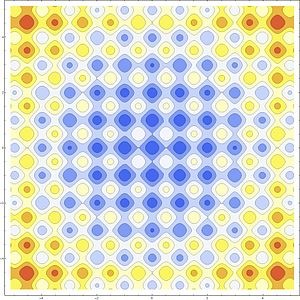
\includegraphics[]{figures/rastagrind}
\caption{Rastrigrins function is a function that is challenging to optimize, as it contains thousands of local optima which would trap a gradient descent algorithm}
\end{figure}
\end{center}

%optimization

Computational optimization techniques are often specific to a particular type of problem rather than being generalized. However, several notable algorithms have solved a wide range of problems including genetic algorithms and stochastic gradient descent (SGD). The popularity of these two algorithms is due to their robustness. Genetic Algorithms and SGD are able to avoid falsely reporting a local minimum when a more optimal solution is available.\\
\\
Stochastic gradient descent, and Genetic Algorithms both utilize concepts like mini-batches, random perturbation (mutation) and combining the concept of average fitness with stochasticity. \\


%to sub-optimal code.\\
%\\

% Move this up to precede a description of specific algorithms.  Multiobjective could apply to gradient descent as well.  You can then refer back to this when you talk specifically about algorithms like NSGA in the "genetic optimization" section.
\subsubsection{Constraints}
A constraint is the implemented mathematical function, very often the function seeks to difference a part of a signal that was sampled with a matching part of a known.
\subsubsection{Multiobjective optimization} Multi objective optimization problems are a subset of optimization problems. In a multiobjective optimisation model fitness is evaluated against multiple constraints rather than just one constraint. 
\\
It is often possible to reduce multiple constraints into one constraint by summing the outputs of objective functions together. There is a price of reducing multiple errors into one error. I will illustrate the problem of multi-objective optimisation. optimization using a sum over multiple error measurements leads to a situation where a single constraint that is easier to satisfy, rapidly drags down the error score and dominates the overall error reading in this manner. In the worst case, the optimizer achieves perfectly low error on one criteria, and high error on a different set of criteria.\\
%by contributing lower errors to the sum of error scores. 
\\
Additionally problems formulated in a multi-objective paradigm are better able to result in diverse solution sets. where multiple and diverse models give satisfactory solutions to the provided constraint, 
\\
However of SGD and NSGA2 only NSGA2 is a natural choice for tackling multi-objective optimization problems. Default implementations of SGD are not able to utilize the principle of non-domination as an optimization strategy.\\
\\
There is a great diversity of real biological neurons, all of which differ substantially in their electrical behavior. There are a few different classes of general purpose neuronal models, that can reproduce these different types of electrical behaviours, given appropriate parameterizations of the models.\newline
\newline
An existing class of neuron model type, called The Izhikevich model \cite{izhikevich2003simple} (Iz model) was published with parameter sets believed to make the model outputs accurately align with a variety of real biological cell outputs. However since publication much very specific electro physiological recordings have accumulated, that in someways undermine model/experiment agreement. However it is now possible to constrain the Izhikevich model and find new parameterizations that more allow us to more accurately reproduce more recently published experimental data.\newline
\newline

% First include a section about NeuronUnit more generally.  NeuronUnit really isn't/wasn't about optimization until your thesis.  
\subsection{Data Fitting and Optimization with NeuronUnit}
A python library "NeuronUnit" provides two functions that help with optimization, these functions are accessible via an API. The first function, is the automatic scaling of model outputs, to match the statistical distribution of observed measurements. For example resting membrane potential is measure in $(mV)$, and it may vary according to a distribution with a mean and standard deviation of $(\mu,\sigma)=(-65mV,15mV)$. Additionally an optimizer may sample a model with a membrane potential of $-67mV$. Neuronunit is able to take these parameters, compute a Z-score, and then compute the $\chi^{2}$
statistic on the collection of normalized Z-scores.\\
\\
In this way NeuronUnit converts a quantitative measure of model/data agreement into a useful error signal. A very natural application of this signal is to guide the process of optimization. The second function of neuronunit is a tool for aggregating relevant experimental data, to construct a formal tests of model fitness. Peripheral to these tools is another module that does some signal processing and feature extraction on the membrane potential waveform. Beyond guiding data fitting, Neuronunit can then evaluate overall model fitness of the optimal model across a variety of appropriate tests.

%  Generalized Linear Integrate and Fire model\cite{teeter2018generalized} or

We have used Neuronunit to guide optimization by taking a flexible model types such as the Izhikevich model and then fitted these models using relevant experimental measurements inside our optimization frame work.

As an example, select Best (IBEA) was used to optimize models in conjunction with data driven tests based on pooled data from NeuroElectro.org \cite{tripathy2014neuroelectro}. A variety of compact and fast single compartment models were used to explore model optimization. Figure 4 demonstrates test error at the beginning of the optimization process for models with randomly sampled parameters and the smaller error following optimization. Figure 5 shows the evolution of the error during the optimization process. \newline
\newline
Optimized neuron models may vary from their neuron counterparts for several reasons. Table 3 shows an example where optimizing the model with respect to the rheobase test comes into conflict with minimizing with respect to input resistance. The solution to the optimization problem consists of two sets of model parameters, which can resolve this conflict differently. Examining the experimental data that these tests were derived from suddenly becomes important. By examining the data, we can see if the rheobase currents and the distributions of input resistance are bi-modal and uniformly distributed. If the data is treated as uni-modal, and the uni-modal mean is used to optimize then the model, then the model is not able to satisfy both constraints simultaneously. In this case, the measurements don’t correspond to neuron data, and the model can’t produce the artificial behavior. When comparing complex data and simple models we find that solutions are better represented using a combination of two optimization solutions.\\
\\
Another potential issue to consider when evaluating the scientific merit of a model is that neurons may have different behaviors under different stimulation paradigms. It might be appropriate to compare modeled behavior against measurements specific to each of two or more distinct modes. In this case, when optimizing single cell models, it’s appropriate to accept a solution set, rather than a single solution. For example, the cerebellar Purkinje cell is sensitive to intricately patterned dendrite input current combinations. Depending on a cell’s recent history of synaptic stimulation, a Purkinje cell may toggle between coincidence detection and integration modes (Ratté, Hong, De Schutter, \& Prescott, 2013).
\\

% I think you can make this section a bit shorter, and refocus to talk about how one major goal is to build tools that can be integrated into the larger modeling ecosystem.  You could have simply written an optimizer in DEAP using jitted python code, custom for each model type, but then you would not be able to interface with everyone else and no one would be able to make use of your tool.  So talk about the importance of standards and interfacing.  and then introduce these tools as standards and components that you need to be able to work with.  
\subsubsection{Ecosystem of Modelling Resources}
The NEURON simulator is a software suite that wraps powerful and fast ordinary differential equation solvers based in the C programming language inside a mixed compiled/interpreted environment targeted at research scientists. NEURON is somewhat analogous to older, analog circuit simulators; however, rather than describing complex resistor-capacitor circuits, NEURON instead solves equations for the time varying membrane potential of multi-compartment models.\\
\\
In contrast to reduced models, multi-compartmental models digitally encode the form of membrane tissue: cables of varying diameters and lengths that represent the morphology of neurons, and these cables support smaller scale representations of ion channels, and ion currents in the membranes. These neuronal models can be coupled together into a network, where the electrical state of one neuron has an impact on the state of coupled neurons through synaptic currents. Specifying the system of differential equations representing these neuronal morphologies, ion channels, and synaptic connections is complicated, but NEURON makes multi-compartment neuron simulation efficient, convenient, and achievable. Models expressed in NEURON code are procedural in nature, and the code consists of low-level implementation details. Procedural descriptions of models are difficult to extend and re-use, leading to a need for a declarative model description language. NeuroML has been tasked with describing these with complex network models.\newline
\newline
%Through jNeuroML, the NeuroML project also provides a simple code interface for generating complex simulator code, so that NeuroML models are readily exchanged between different types of simulators. Model interchange permits cross examination of results as a they vary across simulators, and this interchange promotes the movement of models between languages preferred by different modeling communities, reconciling and unifying their models. Because NeuroML is extensible and component based, it incentivizes a "plug\-in" environment for including pre\-existing model components in models in a different large-scale context.

% illustrate how a Genetic Algorithm (GA) generally works.
\begin{center}
\begin{figure}
    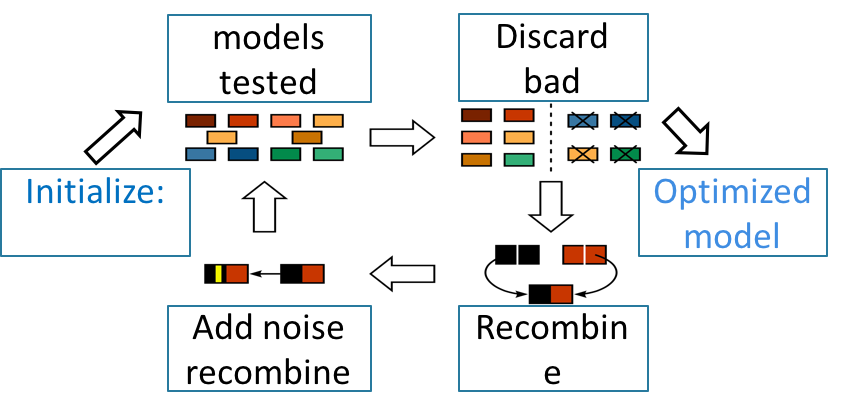
\includegraphics[width=0.7\linewidth]{figures/How_Genetic_Alg_Works.png}
  \caption{Genetic Algorithm Overview}
  \label{fig:GeneticAlgOver}
\end{figure}
  
\end{center}

In \ref{fig:GeneticAlgOver}  Genetic algorithms find satisfactory solutions by incompletely sampling the solution space. Evolution of the algorithm is guided by the combined application of stochastic sampling and selective pressure. Stochastic contributions that guide GA sampling incentivise the exploration of regions beyond local minima. Stochasticity is applied in the combined actions of cross-over, and mutation. Model parameterizations are encoded as binary strings called genes. When genes breed, eligible pairs of genes are aligned and at random bit locations, the status of a bit is exchanged.  

%\subsection{Significance}
% I wouldn't call this section "Significance".  In general, think of these sections as small modules that can be reshuffled and rearranged as needed.  You don't want to pin yourself to describing everything that is "Significant" right here.  In particular, you could call this section "Neuronal diversity".

\subsection{Analysis of Model and Experimental Variance}
Beyond experimental error, it is common to observe large variations in measurements of a single electrophysiological entity from neurons of the same classification. In another section %\href 
Results I visualization such variation in electrophysiological measurements. As an example, consider that measurements of neuron membrane input resistance may be different when recorded from different instances within the same neuron type. Within sample variation is an essential consideration when evaluating the scientific merit of a computational model of a neuron-type. In conjunction to optimization, we propose to perform a large-scale analysis of model against experiment agreement and model against model agreement to expose the variation in biophysically realistic neuron models and cortical data.\\
\\
By analyzing the variance in experiments and models the heterogeneity of experimental measurements from a particular neuron-type. Performing a meta-analysis with a large number of models will provide other insights. We will determine whether there is higher variance in modeled electrical properties versus experimental neurophysiological measurements. We will examine whether an extensive collection of cortical models behaves more similarly to each other than to the data and will answer the question: does the space of all existing single cell models accurately represent the variability in experimental data?\\
% I didn't do this in thesis work.
%and linking the variation to specific features and mechanisms, 
%we also will better understand 
%Similarly, variation in the behavior of cortical neuronal networks is not well quantified. Tremendous research effort has been consumed producing several high-quality, experimentally informed cortical network models. Before creating another elaborate network model, we will determine whether these pre-existing approaches lead to networks with significantly different dynamic properties. Also, we will create an infrastructure that allows scientists to quantify the similarities and differences among networks and their dynamics – both biological and in silico.\newline
\newline
% Shouldn't this be a new section, about data integration?
\subsection{Relationship between Missing Data Imputation and Optimization}
Existing data sets are incomplete, consisting of a sparse sampling of cells in the rodent brain. By necessity, models are constrained using these incomplete data sets, leading to compensatory model development that synthesizes missing information. Missing data occurs at multiple levels during network construction including exact neuron to neuron wiring patterns, un-sampled morphologies, unknown synapse activation times, and unknown axon and dendrite synapse locations. Published models should not be regarded as final, but to improve models, it is vital that they are validated against newly-obtained experimental data. The proposed work will facilitate ongoing validation of biophysically realistic models. 
\\
% And this can go up into the section about diversity
Some electrophysiology data are challenging to integrate into existing models. These include data collected from animal species that are not widely used in models such as marmoset, guinea pig, and even humans.  Rarely, neuon-type data may come from a human, but the tissue samples will have been extracted from pathological brain tissue pertaining to conditions, such as eplipsey or Alzheimers disease.
\\
In practice, open access data is not always useable, as it be derived from multiple species, multiple brain regions and different states of health. We will obtain a better understanding of region-dependent differences and species-dependent differences in order to help researchers map models onto a standardized rodent electrophysiological phenotype space.\\
\\
\subsection{Distinction of Optimization Approach From Other Approaches}
% This can be a fusion of your sections about multiobjective optimization, unit testing, and data integration (or whatever set of background items you think is fundamental to understanding the novelty of the work you have done).
Please elaborate on these limitations in a section called 



\subsection{Distinction of Large Scale Analysis From Other Approaches}
The large-scale meta-analysis described here has not been performed previously. For the first time, a large number of cortical neuron and neuronal network models are available in the standardized NeuroML format. Although the Allen Institute for Brain Science modeling project and the Blue Brain project both rigorously analyzed their single cell models, to the best of my knowledge there has not been an overarching meta-analysis across different cell and network model sources.\\
\\
Similarly, numerous modeling efforts have employed data-driven testing in model development workflows, but all these efforts have been based on non-standard ‘in-house’ model types and execution environments. In contrast, this work proposes to expand a pre-existing standardized model testing space, NeuronUnit, that supports model validation and re-use regardless of the model source. To date various NeuronUnit tests of action potential shape, electrical properties, and single cell morphologies exist; yet these tools are not unified. Some tests of network dynamics also currently exist; however, these tests are not integrated into a unified multiscale workflow. Although the work I describe only concerns single cell models in isolation, significantly, a unified workflow for exploring model data agreement would better locate errors in network behavior which are manifest at the network level but are caused by neuron-type models. \newline
\newline

\chapter{Introduction}

\subsection*{Motivation for Reduced Models of electrically excitable cortical cells}

Multi-compartment conductance based models consist of fine grained biophysical models of neuron membrane including ion channel conductance, and membrane shape and form. These biophysical models take a significant time and computer resources to evaluate. A different class of neuronal model, known as a "Reduced model" is comparatively fast to solve. Speed, empirical validity, are among the two biggest constraints affecting the design of cortical brain models. 
% Further more reproducibility and accessibility are increasingly regarded as important model design constraints too., and they will also be addressed in this work. 

Brief duration model evaluations are critical to brain network simulation speed, as each of many models must be evaluated synchronously according to a global network clock, and there is a high dependency between the states of different models. Network simulation is only as fast as the slowest model, because (if you are waiting for one neuron to evaluate, the whole network will need to wait, as its state may depend on that neuron). Since these constraints are in direct conflict with each other, many scientists are interested in the finding the most optimal resolution to this speed/accuracy trade-off.\\ 
\\
The work herein is aligned with one particular approach to the trade-off. To make data specific versions of simpler models, such that simpler models better mimic experimentally observed electrical measurements. To understand this approach to improving model speed and accuracy, it is important to be familiar with the concept of reduced neural models. Some types of neural models are mimic neurons across many different forms and scales.\\
\\
This approach contrasts with other existing approaches to neuronal model optimization. Shape, and ephysiology based approach in contrast to a spike timing approach. 
\\
Examples of reduced models are:
Point conductance based model, Adaptive Exponential Integrate and Fire model, and Izhikevich model, and in fact, these are the only reduced models considered in the scope of this document.\\
\\
These models are easier faster to evaluate, but they are also easier to understand.

% I will discuss each different model in its own section.
\subsubsection{Importance of Simulation Duration}
The speed of cell-model evaluation is a critical factor for gaining scientific insight from brain simulations. At the network, or mesoscopic level of description, and  microscopic features to simulations significantly slows simulation speed. Even when using High Performance Computing developing simulations involves a debugging errors in different modalities, sometimes the computer program needs correcting, but at other times the scientific expectations about neural dynamics might be wrong. The maths might be wrong. To correct for any mistakes, feedback in the form of observed model behavior, is essential, for the development of the model itself, and short simulation durations are critical to this.\\
\\
The are several valid instances when the complete three dimensional form of a neuron is an integral part of a brain simulation, such as in the Blue Brain somato-sensory cortex model \cite{markram2006blue} and the Allen Institute $V1$ model \cite{billeh2020systematic}, These simulations are improved by encasing a "core" of biophysically accurate models inside a "shell" of simple fast and reduced Izhi, GLIF, or AdExp models.\\ 
\\
Encasing a core of complex models inside a shell of simplified models mitigates an observable "edge effect" problem. The problem is that simulations concern sub divisions of brain tissue, subdivisions by nature exclude externally sourced synaptic inputs. These synaptic inputs are connections that are severed by the process of making a subdivision. All published highly detailed simulations to date, have necessitated the simulation of severed volumes of tissue, and this creates another problem to manage.\\
%There is a core of models of realistic models who are missing a substantial number of "extrinsic" synaptic inputs. 
Almost all cortical neurons experience "tonic" synaptic input and these tonic inputs originate from neurons from a different part of the brain. One strategy for handling inputs that are external to the region of interest, is to simply model spike trains for each input synapse. Modern programming languages have tools that can make matching the synthesis of statistically similar spike trains convenient. One big problem with this approach is it assumes that post synaptic neurons are mainly influenced by the firing rate of inputs, if they pre-synaptic neurons are actually conveying important code words via exact interspike intervals, a statistical approach to modelling spike trains would not do.\\

%An alternative approach is to reduce the complexity of neural models as one exceeds the boundary of the region of interest.

%than generating only psuedo random timed inputs to synapses, 
In the case of the Allen Institute Model, if the region of interest V1 is a "core" of realistic neurons. That is a kernel of realistic neurons encased by a shell of less realistic neurons. Inputs to V1 also come from the outer encasement of neurons. It is therefore of interest if these external GLIF models can or should be substituted with optimized Izhikivich and AdExp models, in case substiting GLIF for Adexp results in an overall more realistic network simulation. In that case, even the external shell of simulation could experience a marginal improvement in accuracy. In network models there are benefits of reduced models over the use of a point process or a spike train surrogate.\\

% benefits: interpretability, transparent function, has current so contributes to LFP

One of these benefits is that the firing of reduced neural models can be made to be causal, such that its spike times are not just what statistically matches missing models. Furthermore reduced models can still participate in networks, reduced models can become disconnected or participate in an dynamic assembley. Realistic levels of plasticity of the modelled network is more possible with included reduced models, than statistical surrogates of those models.

Furthermore Izhikivitch and AdExp models are commonly utilized in neuromorphic spiking neural networks in artificial intelligence and bio medical modelling contexts.
%archictecture.

%\subitem 
optimization is an interaction between models and constraints which guides a fitting process. Not all neural models are equally flexible.  
%\item  
Both the choice of constraining equations, and the choice of neural models must be favorable in order for models to be fitted to data.
%\item 
%\subitem 
if the combination of models and constraints is bad, then then a tractible error surface will not result.  

%\subsubitem 
Unfortunately, it is not always possible to know without trying which combinations of \subitem[A]: models, and \subitem[B], constraints will lead a tractable error surface, however a nicely smooth manifold surface with only minor oscillations is preferable

%that a Genetic Algorithms can use to find a global solution to. As an example consider  

I describe some code implementation experiments were the model/constraint combination lead to DEAP genetic algorithms matching model parameters to constraints and model/constraint selections that lead to optimizer performing only marginally better than a random search of parameter space\\
\\
%\item 
If the number of dimensions that are searched exceeds the degree and the effectiveness of constraints, then model optimization is only slightly better than random sampling of solution space.

\subsubsection{Successful Optimization} 
Successful Optimization is more likely to occur if a favorable combination of models and objective functions occured. 
%\item 
The exact way, that model constraint combinations interact cannot always be known in advance, and yet the interaction can be assessed by attempting to optimize on the pair. Experimenting of model test combinations is what was done in this body of work.

It is important to note that, the measurements that are built off something that is relative to another changeable quality in a model are prone to resonance and oscillation. For example measuring $ \frac{1}{10} \times \frac{dv}{dt} $

Efficient model examples: (generalized leaky integrate and fire model) GLIF, Izhikitch. Adaptive Exponential Integrate and fire model, single compartment conductance based model. 

%\item 
There are at least three different and com-possible approaches to more realistic brain simulations. In one approach you would make biophysically accurate models faster. In a different approach you could make reduced models more accurate. To make reduced models more accurate, you would find parameterizations of the models that let the models act as better mimics of experiments.
%\item 
%Herein we investigate how well Faster models can match experimental recording waveform shapes.
%\item 
%The reason why we want to investigate the match:
%\item 
%Large scale simulations cant evaluate on a timescale that is meaningful, unless a large ratio of modelled cells are "reduced models"
%\item 
%Reduced Models already enjoy wide spread usage. We want to investigate if reduced models can be made to be more realistic, by checking if they can mimic data better.
%\item 
%If reduced models can't be made more realistic (herein we show only marginal improvements), we need to show the limitations of reduced cells, with regards to a particular set of tests.
%\item
%We need to document the approach used, and how the approach contrasts with spike time approaches to model fitting.
%\end{itemize}

\subsubsection{Optimizing multispiking Behavior}

When using Allen experimental data to create multi-spiking tests, there was the potential to more tightly constrain model behavior. In order to evaluate the goodness of fit models the $Chi^{2}$ statistic could no longer be used, instead one could compute the 'variance explained ratio' between the allen institute experimental sweep and the optimized models sweep to a comparable current injection.

and there is also the potential to check the variance explained ratio of tests.
In such a multispiking paradigm the highest possible variance explained ratio of approx $1$. 

Caption in this figure there is visibly almost perfect  agreement between simulated and experiments and the optimized models, in the passive experimental conditions, and a close match for the spiking model behavior. There was a standard suite of tests if only spike-half-width, not spike-base-width. The Izhi models width as thus free to vary at the base, take that into account when eye balling the two graphs and you can see why almost binary match. EFEL does achieve spike width binary matching because it uses both half-width, and base-width. If you look at the last cells you can see I take a correlation matrix of the optimizers errors over its history. The idea is if it's normalized then I can sum the whole matrix and get a single scaler number to show how de-correlated both error sets are over the GA evolution. 

It was found that the elephant/neuroelectro-suite of NU tests don't fully constrain the spike width at the base of neuron action potential waveform. Since the base of the waveform was unconstrained, it was free to vary, half-spike-width is constrained, it is more appropriate to talk about variance explained of the spike snippet. $variance explained>0.95$ is a useful heurism. Allowing some margin acknowledges that we shouldn't assume we have represented all waveform features that can vary. If you want variance explained ==1   you could optimize using a variance explained cost function, but we don't want to do that.

%\begin{itemize}
%\item 
%First with $2$ constraints, then with $>100$ constraints via the feature extraction suite EFEL

%\item 
%This is a two staged approach. 
%\item 
%It uses three step protocols.

%\item 

%\item 
%In this two stage algorithm: I optimize, using constraints: spike count at injection strength $1.5 \times rheobase $, and $3.0 \times rheobase $
%I do a quick check of spike counts at 1.5 and 3.0 rheobase (2 constriants only).
%\item 
%In this scenario Rheobase is used only as a soft constraint. Firstly we optimize the model to spike count data we very rapidly narrow down the solution space using only two errors. \\
%\\
%In a second code experiment I use the standard NU suite, for a lot of generations. In the figure below
%%
% Figure
%%
 
%\end{itemize}


% Add a section about model databases and the opportunities they will make available to you.  Describe how we don't really know whether the models in these databases match the experimental data they claim to recapitulate.  Describe some of the specific challenges in using "in house" data.